\documentclass[tikz,border=10pt]{standalone}
\usepackage{helvet}
\renewcommand{\familydefault}{\sfdefault}
\usepackage{amsmath}
\usepackage{bm}
\usetikzlibrary{arrows.meta, positioning, fit, calc, shapes.geometric, decorations.pathmorphing, backgrounds}

\definecolor{emeraldpine}{HTML}{1A4D3E}
\definecolor{harvardcrimson}{HTML}{A51C30}
\definecolor{ethdarkblue}{HTML}{1F407A}
\definecolor{ethpetrol}{HTML}{007A87}
\definecolor{ethbronze}{HTML}{B87333}
\definecolor{ethpurple}{HTML}{5B4B8A}
\definecolor{ink}{HTML}{1A202C}
\definecolor{softink}{HTML}{4A5568}
\definecolor{paleink}{HTML}{A0AEC0}
\definecolor{cardbg}{HTML}{F8FAFC}
\definecolor{shadecolor}{HTML}{F4F6F9}

\definecolor{panel1light}{HTML}{EFF6FF}
\definecolor{panel1border}{HTML}{BFDBFE}
\definecolor{panel2light}{HTML}{FEF2F2}
\definecolor{panel2border}{HTML}{FECACA}
\definecolor{panel3light}{HTML}{FFFBEB}
\definecolor{panel3border}{HTML}{FDE68A}

\begin{document}
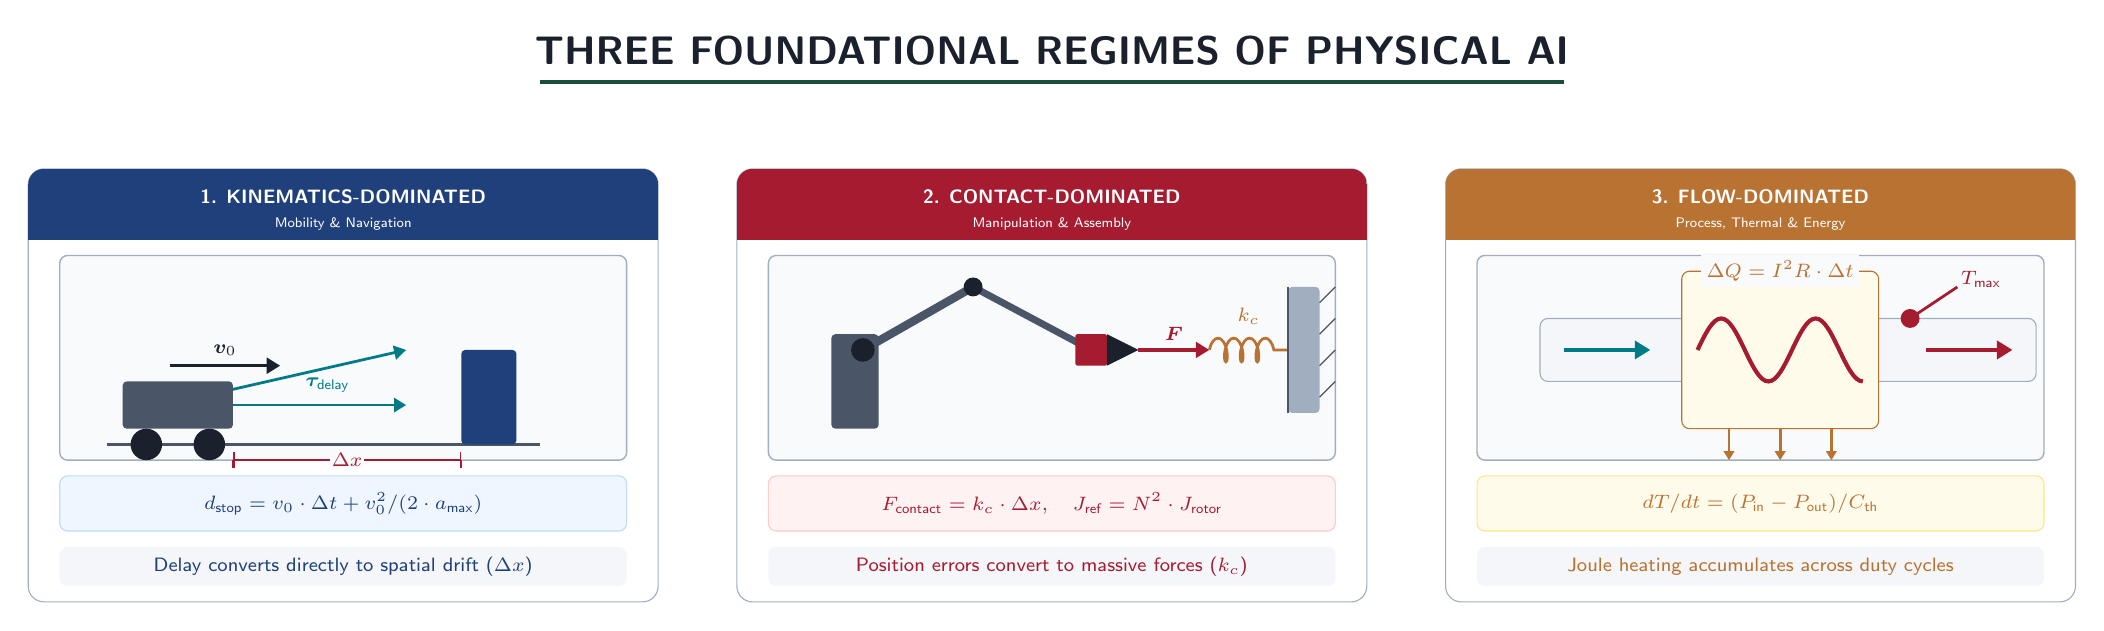
\begin{tikzpicture}[x=1mm, y=1mm]
  \node[font=\sffamily\bfseries\Large, text=ink] at (130, 70) {THREE FOUNDATIONAL REGIMES OF PHYSICAL AI};
  \draw[emeraldpine, line width=1.5pt] (65, 66) -- (195, 66);

  % PANEL 1
  \begin{scope}[shift={(0,0)}]
    \draw[draw=paleink, fill=white, rounded corners=2mm] (0,0) rectangle (80, 55);
    \clip[rounded corners=2mm] (0,0) rectangle (80, 55);
    \fill[ethdarkblue] (0, 46) rectangle (80, 55);
    \node[text=white, font=\sffamily\bfseries\scriptsize] at (40, 51.5) {1. KINEMATICS-DOMINATED};
    \node[text=white, font=\sffamily\tiny] at (40, 48) {Mobility \& Navigation};

    \fill[cardbg, rounded corners=1mm, draw=paleink, line width=0.5pt] (4, 18) rectangle (76, 44);
    
    % Panel 1 Schematic
    \begin{scope}[shift={(10, 20)}]
      % Floor
      \draw[softink, line width=0.8pt] (0, 0) -- (55, 0);
      % Robot Base
      \fill[softink, rounded corners=0.5mm] (2, 2) rectangle (16, 8);
      % Wheels
      \fill[ink] (5, 0) circle (2);
      \fill[ink] (13, 0) circle (2);
      % Sensor Ray
      \draw[ethpetrol, line width=1pt, -{Triangle[scale=0.8]}] (16, 7) -- (38, 12);
      \draw[ethpetrol, line width=1pt, -{Triangle[scale=0.8]}] (16, 5) -- (38, 5);
      \node[text=ethpetrol, font=\sffamily\scriptsize] at (28, 7.5) {$\bm{\tau}_{\text{delay}}$};
      
      % Obstacle
      \fill[ethdarkblue, rounded corners=0.5mm] (45, 0) rectangle (52, 12);
      
      % Velocity vector
      \draw[ink, line width=1.2pt, -{Triangle[scale=0.8]}] (8, 10) -- (22, 10);
      \node[text=ink, font=\sffamily\scriptsize, above] at (15, 10) {$\bm{v}_0$};
      
      % Stopping distance markers
      \draw[harvardcrimson, line width=0.6pt, dashed] (16, -3) -- (16, -1);
      \draw[harvardcrimson, line width=0.6pt, dashed] (45, -3) -- (45, -1);
      \draw[harvardcrimson, line width=0.6pt, {Bar[width=2mm]}-{Bar[width=2mm]}] (16, -2) -- (45, -2);
      \node[text=harvardcrimson, font=\sffamily\scriptsize, fill=cardbg, inner sep=0.5pt] at (30.5, -2) {$\Delta x$};
    \end{scope}

    % Formula Box
    \fill[panel1light, rounded corners=1mm, draw=panel1border] (4, 9) rectangle (76, 16);
    \node[text=ethdarkblue, font=\sffamily\scriptsize] at (40, 12.5) {$d_{\text{stop}} = v_0 \cdot \Delta t + v_0^2 / (2 \cdot a_{\text{max}})$};

    % Bottom Takeaway
    \fill[shadecolor, rounded corners=1mm] (4, 2) rectangle (76, 7);
    \node[text=ethdarkblue, font=\sffamily\scriptsize] at (40, 4.5) {Delay converts directly to spatial drift ($\Delta x$)};
  \end{scope}

  % PANEL 2
  \begin{scope}[shift={(90,0)}]
    \draw[draw=paleink, fill=white, rounded corners=2mm] (0,0) rectangle (80, 55);
    \clip[rounded corners=2mm] (0,0) rectangle (80, 55);
    \fill[harvardcrimson] (0, 46) rectangle (80, 55);
    \node[text=white, font=\sffamily\bfseries\scriptsize] at (40, 51.5) {2. CONTACT-DOMINATED};
    \node[text=white, font=\sffamily\tiny] at (40, 48) {Manipulation \& Assembly};

    \fill[cardbg, rounded corners=1mm, draw=paleink, line width=0.5pt] (4, 18) rectangle (76, 44);
    
    % Panel 2 Schematic
    \begin{scope}[shift={(10, 20)}]
      % Base
      \fill[softink, rounded corners=0.5mm] (2, 2) rectangle (8, 14);
      % Link 1
      \draw[softink, line width=3pt, line cap=round] (6, 12) -- (20, 20);
      \fill[ink] (6, 12) circle (1.5);
      % Link 2
      \draw[softink, line width=2.5pt, line cap=round] (20, 20) -- (35, 12);
      \fill[ink] (20, 20) circle (1.2);
      % Wrist Force Sensor
      \fill[harvardcrimson, rounded corners=0.2mm] (33, 10) rectangle (37, 14);
      % End Effector
      \fill[ink] (37, 10) -- (41, 12) -- (37, 14) -- cycle;
      
      % Force vector
      \draw[harvardcrimson, line width=1.2pt, -{Triangle[scale=0.8]}] (41, 12) -- (50, 12);
      \node[text=harvardcrimson, font=\sffamily\scriptsize, above] at (45.5, 12) {$\bm{F}$};
      
      % Spring compliance model
      \draw[ethbronze, line width=1pt, decoration={coil, aspect=0.4, segment length=2mm, amplitude=1.5mm}, decorate] (50, 12) -- (60, 12);
      \node[text=ethbronze, font=\sffamily\scriptsize, above] at (55, 14) {$k_c$};
      
      % Rigid Wall
      \fill[paleink, rounded corners=0.5mm] (60, 4) rectangle (64, 20);
      \draw[softink, line width=0.5pt] (60,4) -- (60,20);
      % Hatching
      \foreach \y in {6, 10, 14, 18} {
         \draw[softink, line width=0.4pt] (64, \y) -- (66, \y+2);
      }
    \end{scope}

    % Formula Box
    \fill[panel2light, rounded corners=1mm, draw=panel2border] (4, 9) rectangle (76, 16);
    \node[text=harvardcrimson, font=\sffamily\scriptsize] at (40, 12.5) {$F_{\text{contact}} = k_c \cdot \Delta x, \quad J_{\text{ref}} = N^2 \cdot J_{\text{rotor}}$};

    % Bottom Takeaway
    \fill[shadecolor, rounded corners=1mm] (4, 2) rectangle (76, 7);
    \node[text=harvardcrimson, font=\sffamily\scriptsize] at (40, 4.5) {Position errors convert to massive forces ($k_c$)};
  \end{scope}

  % PANEL 3
  \begin{scope}[shift={(180,0)}]
    \draw[draw=paleink, fill=white, rounded corners=2mm] (0,0) rectangle (80, 55);
    \clip[rounded corners=2mm] (0,0) rectangle (80, 55);
    \fill[ethbronze] (0, 46) rectangle (80, 55);
    \node[text=white, font=\sffamily\bfseries\scriptsize] at (40, 51.5) {3. FLOW-DOMINATED};
    \node[text=white, font=\sffamily\tiny] at (40, 48) {Process, Thermal \& Energy};

    \fill[cardbg, rounded corners=1mm, draw=paleink, line width=0.5pt] (4, 18) rectangle (76, 44);
    
    % Panel 3 Schematic
    \begin{scope}[shift={(10, 20)}]
      % Pipe
      \fill[shadecolor, rounded corners=1mm, draw=paleink] (2, 8) rectangle (65, 16);
      
      % Flow Arrows
      \draw[ethpetrol, line width=1.5pt, -{Triangle[scale=0.8]}] (5, 12) -- (16, 12);
      \draw[harvardcrimson, line width=1.5pt, -{Triangle[scale=0.8]}] (51, 12) -- (62, 12);
      
      % Heat Source
      \fill[panel3light, rounded corners=1mm, draw=ethbronze] (20, 2) rectangle (45, 22);
      % Coil
      \draw[harvardcrimson, line width=1.5pt] (22, 12) sin (25, 16) cos (28, 12) sin (31, 8) cos (34, 12) sin (37, 16) cos (40, 12) sin (43, 8);
      
      % Heat Dissipation
      \draw[ethbronze, line width=1pt, -{Triangle[scale=0.6]}] (26, 2) -- (26, -2);
      \draw[ethbronze, line width=1pt, -{Triangle[scale=0.6]}] (32.5, 2) -- (32.5, -2);
      \draw[ethbronze, line width=1pt, -{Triangle[scale=0.6]}] (39, 2) -- (39, -2);
      
      % Thermocouple
      \fill[harvardcrimson] (49, 16) circle (1.2);
      \draw[harvardcrimson, line width=1pt] (49, 16) -- (55, 20);
      \node[text=harvardcrimson, font=\sffamily\scriptsize] at (58, 21) {$T_{\text{max}}$};
      
      \node[text=ethbronze, font=\sffamily\scriptsize, fill=cardbg, inner sep=2pt] at (32.5, 22) {$\Delta Q = I^2 R \cdot \Delta t$};
    \end{scope}

    % Formula Box
    \fill[panel3light, rounded corners=1mm, draw=panel3border] (4, 9) rectangle (76, 16);
    \node[text=ethbronze, font=\sffamily\scriptsize] at (40, 12.5) {$dT/dt = (P_{\text{in}} - P_{\text{out}}) / C_{\text{th}}$};

    % Bottom Takeaway
    \fill[shadecolor, rounded corners=1mm] (4, 2) rectangle (76, 7);
    \node[text=ethbronze, font=\sffamily\scriptsize] at (40, 4.5) {Joule heating accumulates across duty cycles};
  \end{scope}

\end{tikzpicture}
\end{document}
